\documentclass[UTF8,a4paper,11pt,fontset=fandol]{ctexart}
\usepackage[margin=2cm]{geometry}
\usepackage{amsmath,amssymb,booktabs,graphicx,float,fancyhdr}
\usepackage[hidelinks]{hyperref}
\pagestyle{fancy}\fancyhf{}
\fancyhead[L]{\small INT6165 ProductRelated 分组深入检查}
\fancyhead[R]{\small 任务 7}\fancyfoot[C]{\thepage}
\setlength{\headheight}{15pt}\setlength{\parskip}{3pt}
\renewcommand{\arraystretch}{1.15}
\begin{document}
\begin{center}{\LARGE\bfseries ProductRelated 分组深入检查}\\[4pt]
{\small 新访客与回访者的购买率比较}\end{center}
\section*{7\quad 按浏览量进行组内比较}
以会话为单位，保留原始重复记录，排除 Other。纳入 12,245 条会话。数据没有访客 ID，所以下文报告的是\textbf{会话数，不是去重人数}。

ProductRelated 合并样本的四分位点为 7、18、38，两类访客使用相同边界，不依据购买结果选点。组内购买率为 $x/n$，区间采用 Wilson 95\% 置信区间。
\begin{center}\small
\begin{tabular}{llrrl}
\toprule 浏览量 & 访客 & 购买 / 会话数 & 购买率 & 95\% CI\\ \midrule
0--7 & 新访客 & 67/482 & 13.90\% & [11.10, 17.28]\% \\
0--7 & 回访者 & 90/2,620 & 3.44\% & [2.80, 4.20]\% \\
8--18 & 新访客 & 160/644 & 24.84\% & [21.66, 28.32]\% \\
8--18 & 回访者 & 273/2,475 & 11.03\% & [9.86, 12.33]\% \\
19--38 & 新访客 & 144/409 & 35.21\% & [30.74, 39.95]\% \\
19--38 & 回访者 & 449/2,603 & 17.25\% & [15.85, 18.75]\% \\
$\geq$39 & 新访客 & 51/159 & 32.08\% & [25.32, 39.68]\% \\
$\geq$39 & 回访者 & 658/2,853 & 23.06\% & [21.55, 24.64]\% \\
\bottomrule\end{tabular}\end{center}
\textbf{小样本提示规则：}$n<30$，或购买数、未购买数任一小于 5。八个单元均未触发，最小单元为最高浏览量组的新访客（159 条会话，购买 51 次）。规则仅作提示，不保证推断假设全部成立。
\begin{figure}[H]\centering
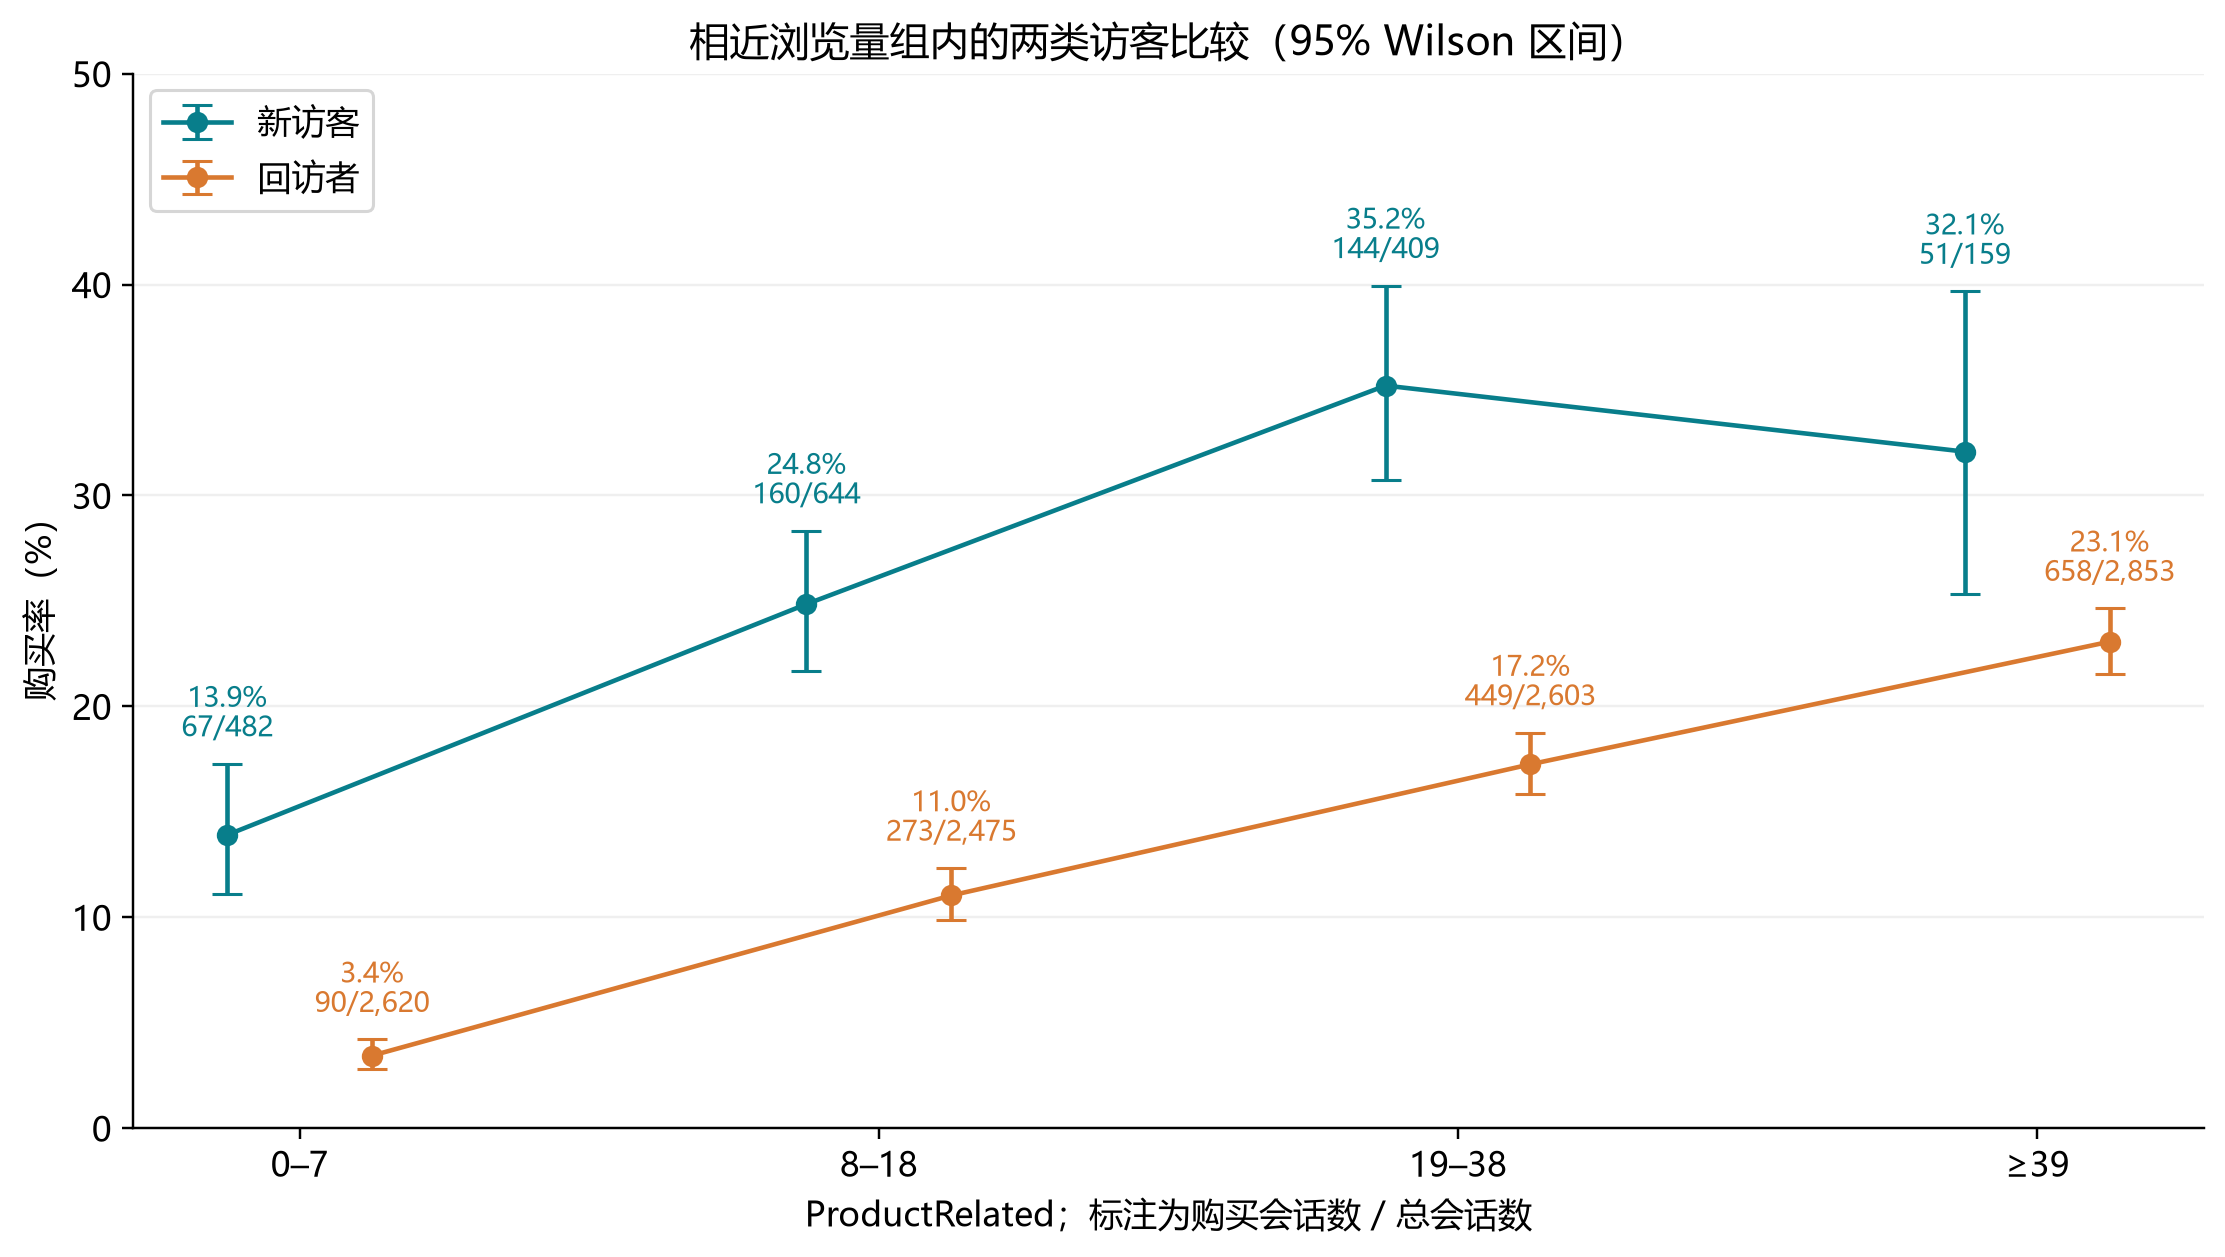
\includegraphics[width=.82\linewidth]{figures/07_group_rates_counts.png}
\caption{组内购买率与 Wilson 区间；标注为购买数 / 会话数}
\end{figure}
\newpage
\section*{7\quad 结果解释与可选 Logistic 回归}
四组中新访客购买率均较高，差值约为 10.47、13.81、17.96、9.01 个百分点。按这一粗略分组口径，差异方向仍在。最高组覆盖 39--705 个页面，不能说已经精确匹配浏览量。各组区间不是同时置信区间，本次不作四次显著性检验，也未检验四组效应是否相同。
\subsection*{两个辅助模型}
设 $N_i=1$ 表示新访客，回访者为基准：
\begin{align*}
\operatorname{logit}(p_i)&=\log\frac{p_i}{1-p_i},\\
\text{模型一：}\quad\operatorname{logit}(p_i)
&=\beta_0+\beta_{\mathrm{N}}N_i+
\sum_{k=2}^{4}\gamma_k\mathbf{1}(G_i=k),\\
\text{模型二：}\quad\operatorname{logit}(p_i)
&=\beta_0+\beta_{\mathrm{N}}N_i+
\gamma\log(1+\mathrm{ProductRelated}_i).
\end{align*}
模型一按四组调整，基准浏览量组为 0--7。模型二用于函数形式敏感性核对，不按 $p$ 值选模型。二者均无交互项，假设新老访客的条件优势比不随浏览量变化。采用最大似然估计及模型标准误，样本量均为 12,245。
\begin{center}
\begin{tabular}{lrrr}
\toprule 调整方式 & 新访客 OR & 95\% CI & $p$ 值\\ \midrule
四组浏览量调整 & 2.639 & [2.314, 3.010] & $<0.001$ \\
log(1+浏览量)调整 & 2.780 & [2.440, 3.166] & $<0.001$ \\
\bottomrule\end{tabular}\end{center}
优势比为 $\exp(\beta_{\mathrm{N}})$，odds 定义为 $p/(1-p)$。
\textbf{OR 不是购买率倍数，也不是增加的百分点。}
两种指定调整方式下均观察到正向关联。主模型已与八单元聚合二项 GLM 核对，系数一致。完整系数及数值 $p$ 值见结果 CSV。
\subsection*{限制}
只调整浏览量，未控制其他变量。ProductRelated 在会话中产生，不能直接视为已确认的前置混杂因素。会话独立性、函数形式和共同优势比假设限制解释。本次没有建立或评估预测模型，也不作因果推断。
\subsection*{可用表述}
“在相同的粗略浏览量组内，新访客购买率均较高；简单 Logistic 调整后方向也一致。”不应表述为“浏览量完全相同时仍有因果效应”。
\end{document}
